% DAMK-Net — LNCS (Springer) manuscript
% Compile on Overleaf with pdfLaTeX. Uses llncs.cls + splncs04.bst (unchanged).
%
\documentclass[runningheads]{llncs}
%
\usepackage[T1]{fontenc}
\usepackage{graphicx}
\usepackage{booktabs}
\usepackage{amsmath,amssymb}
\usepackage{microtype}
\usepackage{tikz}
\usepackage{hyperref}
\usetikzlibrary{positioning,arrows.meta,fit,backgrounds}
\usepackage{pgfplots}
\pgfplotsset{compat=1.18}
%
\newcommand{\cmark}{\ensuremath{\checkmark}}
\newcommand{\xmark}{\ensuremath{\times}}
%
\begin{document}
%
\title{DAMK-Net: Multi-Task Network for Breast Ultrasound Classification and Segmentation}
\titlerunning{DAMK-Net: Compact Multi-Task Breast Ultrasound}
%
\author{Quang Le\inst{1,2}\orcidID{0009-0003-4616-7885} \and Huy Le\inst{1,2} \and Hanh Tran\inst{1,2}}
\authorrunning{Quang Le et al.}
\institute{Faculty of Information Technology, University of Science, Ho Chi Minh City, Viet Nam
 \and Vietnam National University, Ho Chi Minh City, Vietnam \\
% \email{25C1505840@student.hcmus.edu.vn}
}


%
\maketitle
%
\begin{abstract}
Breast ultrasound computer-aided diagnosis needs both lesion segmentation and
benign\slash malignant\slash normal classification, yet lightweight networks usually do one
task and drop normal (non-tumor) scans, while the multi-task methods that keep
normal rely on heavy backbones. We present the \textbf{D}epthwise-separable
\textbf{A}ttention \textbf{M}ulti-\textbf{K}ernel Network (DAMK-Net), a compact
multi-task network that classifies and segments a scan in one forward pass and
keeps normal images throughout. It pairs a depthwise-separable attention encoder with a
multi-kernel attention decoder, and a single width multiplier produces a family
of models from 0.63M to 8.5M parameters. Correct behavior on normal scans comes
from class-balanced oversampling during training together with an inference-time
step that enforces agreement between the two output heads. On the BUSI dataset,
the 2.25M-parameter DAMK-Net-S reaches 85.83\% classification accuracy, above a
dedicated classifier, and 79.4\% lesion Dice, on par with a dedicated segmenter,
while using fewer parameters and FLOPs than running the two models separately. An
ablation confirms, now within a lightweight scalable model, that multi-task
training alone leaves segmentation Dice on normal scans at 0.43 and that the
inference step raises it to 0.90, and shows that the multi-kernel decoder
segments better than an inception-style decoder at a seventh of the compute.
DAMK-Net delivers a complete, deployable breast-ultrasound pipeline in one small
model.

\keywords{Breast ultrasound \and Multi-task learning \and Lightweight neural
network \and Image segmentation \and Image classification \and Computer-aided
diagnosis.}
\end{abstract}
%
\section{Introduction}
Breast cancer is the most commonly diagnosed cancer in women worldwide
\cite{Globocan}, and ultrasound is a standard screening tool because it is
non-ionizing, inexpensive, and works well on dense breast tissue
\cite{BUSI,Survey}. Reading a breast ultrasound scan involves two decisions made
together: whether a lesion is present and where it lies, and whether the tissue
is benign, malignant, or normal. A computer-aided diagnosis (CAD) system that
assists radiologists has to answer both.

Most deep learning methods answer only one. Lightweight segmentation networks
such as MK-UNet \cite{MKUNet}, CMUNeXt \cite{CMUNeXt}, and UltraLight VM-UNet
\cite{VMUNet} reach high Dice scores with very few parameters, but they are
trained and tested only on images that contain a tumor; normal scans are dropped
from the data. Classification networks such as MedNet \cite{MedNet} label the
scan but return no mask. Deploying a full pipeline then requires two separate
models, which doubles the parameter and compute budget on exactly the
point-of-care hardware these compact methods target.

Discarding normal scans is not a small simplification. A substantial share of
screening images contain no lesion, and a model that has never seen a normal
case will mark healthy tissue as a tumor. Aumente-Maestro et al. \cite{CMPB}
argue that handling normal images is what separates a research prototype from a
clinically usable system, and they report that naive multi-task learning fails
badly on this class. Their framework handles it, but it is built on heavyweight
UNet++ and nnU-Net backbones. What is missing is a single network that is small
enough to deploy, performs both tasks, and treats normal as a first-class
category instead of removing it.

We study this problem with the \textbf{D}epthwise-separable \textbf{A}ttention
\textbf{M}ulti-\textbf{K}ernel Network (DAMK-Net), a compact multi-task network
that classifies and segments a breast ultrasound scan in one forward pass and
keeps normal images in both training and evaluation. The network pairs a depthwise-separable
attention encoder with a multi-kernel attention decoder, and a single width
multiplier produces a family of models from 0.63M to 8.5M parameters. To make the
model behave correctly on normal scans, we combine class-balanced oversampling
during training with an inference-time step that enforces agreement between the
classification and segmentation heads.

One design choice deserves explanation up front. Aumente-Maestro et al.
\cite{CMPB} showed, on heavyweight UNet++ and nnU-Net backbones, that multi-task
training by itself fails on the normal class and that a coherence step between
the two heads recovers it. We confirm that this holds in the lightweight,
width-scalable regime: multi-task training alone leaves segmentation Dice on
normal scans at 0.43, and the coherence step raises it to 0.90. The mechanism is
not ours, but the result that it remains necessary in a compact model is what
shapes the design, and we quantify each component's contribution.

\medskip\noindent\textbf{Contributions.}
\begin{enumerate}
\item A unified, width-scalable multi-task network for breast ultrasound that
classifies and segments in one model and keeps normal scans, released as a family
spanning 0.63M to 8.5M parameters.
\item Confirmation, in a lightweight and width-scalable model, of the prior
finding \cite{CMPB} that multi-task learning alone is insufficient for the normal
class and that an inference coherence step is decisive, with an ablation that
quantifies the separate contributions of training-time oversampling and
inference-time prediction-refining.
\item A decoder comparison on a shared encoder: the multi-kernel decoder gives
better lesion segmentation at roughly 6.8 times fewer FLOPs than an
inception-style decoder.
\item On the BUSI dataset, the 2.25M-parameter DAMK-Net-S reaches the accuracy of
a dedicated classifier and the Dice of a dedicated segmenter while using fewer
parameters and FLOPs than running the two separately, and it handles the normal
scans that single-task segmenters leave out.
\end{enumerate}

\section{Related Work}
\subsection{Lightweight segmentation of medical images}
The U-Net encoder-decoder with skip connections \cite{UNet} is the basis for most
medical image segmentation, and many variants add attention or nested skips
\cite{AttnUNet,UNetpp}. These models are accurate but large. For breast
ultrasound specifically, where boundaries are blurred and speckle is heavy,
methods add domain attention or transformer modules, such as a global guidance
network \cite{GGN} and the hybrid CNN-transformer HCTNet \cite{HCTNet}. A separate
line of work targets point-of-care deployment by cutting parameters and FLOPs:
UNeXt \cite{UNeXt} mixes convolutional and MLP blocks, CMUNeXt \cite{CMUNeXt} uses
large-kernel convolutions, and MALUNet \cite{MALUNet}, EGE-UNet \cite{EGEUNet},
and UltraLight VM-UNet \cite{VMUNet} bring parameter counts below 0.1M. MK-UNet
\cite{MKUNet} reports the best accuracy-efficiency trade-off in this group at
0.32M parameters, replacing standard convolutions with multi-kernel depthwise
blocks and adding gated and local attention in the decoder. All of these networks
do segmentation alone. On breast ultrasound they are also evaluated only on
tumor-bearing images: MK-UNet, for instance, uses the 647 benign and malignant
BUSI scans and removes the 133 normal ones.

\subsection{Breast ultrasound classification}
Classifying breast ultrasound into benign, malignant, and normal has been done
with standard CNNs and, more recently, with compact attention-augmented designs.
MedNet \cite{MedNet} stacks residual depthwise-separable blocks with CBAM
attention \cite{CBAM} and reaches competitive accuracy on several medical-imaging
benchmarks at 3.27M parameters, and transformer-based classifiers such as
HoVer-Trans \cite{HoVerTrans} add global context for region-of-interest-free
diagnosis. A classifier outputs a label but no localization, so it cannot stand
in for segmentation in a CAD pipeline.

\subsection{Multi-task learning for breast ultrasound}
A smaller set of methods classifies and segments together to use the correlation
between the tasks: a malignant region should be both outlined and labeled. Zhou
et al. \cite{Zhou}, DBL-Net \cite{DBL}, and ACSNet \cite{ACSNet} share an encoder
across task-specific branches and report strong joint results, but they classify
in the binary benign\slash malignant setting, remove normal scans, and run on
heavyweight backbones; ACSNet, for example, reports 42.99M parameters and 30.96
GFLOPs. Regional and attention-guided variants, including RMTL-Net \cite{RMTLNet},
SHA-MTL \cite{SHAMTL}, and a hybrid CNN-transformer multi-task model
\cite{Shareef}, couple the two tasks more tightly but stay in the same binary,
tumor-only regime. The method of Aumente-Maestro et al. \cite{CMPB} comes closest
to a clinically complete system: it keeps normal images, adds a deterministic
oversampling step for class balance and a prediction-refining step that forces
the two heads to agree, and it shows that plain multi-task learning collapses on
the normal class without these additions. Its backbones, UNet++ and nnU-Net, are
large. MA-DTNet \cite{MADTNet} is lighter and multi-task but classifies in the
binary setting and does not address normal scans.

No prior method is lightweight, scalable, and clinically complete at once. We take
the normal-handling idea from \cite{CMPB} but place it inside a compact,
width-scalable architecture and measure how much each part of it contributes.

\section{Method}
\subsection{Overview}
DAMK-Net has three parts: an encoder shared by both tasks, a classification head,
and a segmentation decoder (Fig.~\ref{fig:arch}). The two tasks place different
demands on the network. Classification needs deep semantic features summarizing
the whole image, which a deep encoder followed by global pooling provides.
Segmentation needs spatial detail at several scales, which a decoder with skip
connections recovers. Sharing one encoder between them is what lets a single
model do the work of two while staying small. Given an input scan, the encoder
produces five feature maps at decreasing resolution. The classification head
reads the deepest map. The decoder rebuilds a full-resolution mask, using the
four shallower maps as skips.

\begin{figure}[t]
\centering
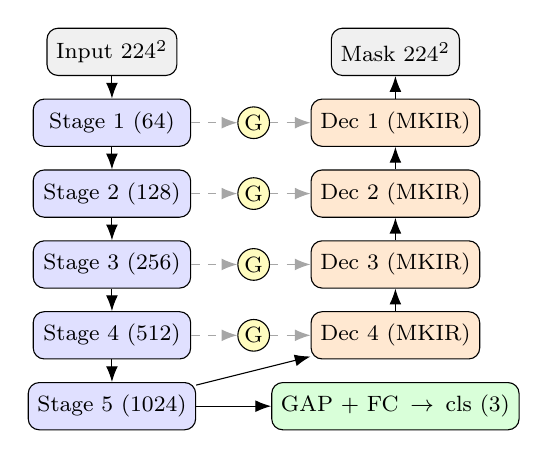
\begin{tikzpicture}[
  font=\footnotesize,
  enc/.style={draw,rounded corners,fill=blue!12,minimum width=20mm,minimum height=6mm},
  dec/.style={draw,rounded corners,fill=orange!18,minimum width=20mm,minimum height=6mm},
  io/.style={draw,rounded corners,fill=gray!12,minimum width=16mm,minimum height=6mm},
  head/.style={draw,rounded corners,fill=green!15,minimum width=22mm,minimum height=6mm},
  gag/.style={draw,circle,fill=yellow!25,inner sep=1pt,minimum size=4mm},
  arr/.style={-{Latex[length=2mm]}},
  skip/.style={-{Latex[length=2mm]},dashed,gray!70}]
% encoder column (left, descending)
\node[io]  (in)  at (0,0)      {Input $224^2$};
\node[enc] (e1)  at (0,-0.9)   {Stage 1 (64)};
\node[enc] (e2)  at (0,-1.8)   {Stage 2 (128)};
\node[enc] (e3)  at (0,-2.7)   {Stage 3 (256)};
\node[enc] (e4)  at (0,-3.6)   {Stage 4 (512)};
\node[enc] (e5)  at (0,-4.5)   {Stage 5 (1024)};
% classification head
\node[head] (cls) at (3.6,-4.5) {GAP + FC \,$\to$\, cls (3)};
% decoder column (right, ascending)
\node[dec] (d4)  at (3.6,-3.6) {Dec 4 (MKIR)};
\node[dec] (d3)  at (3.6,-2.7) {Dec 3 (MKIR)};
\node[dec] (d2)  at (3.6,-1.8) {Dec 2 (MKIR)};
\node[dec] (d1)  at (3.6,-0.9) {Dec 1 (MKIR)};
\node[io]  (out) at (3.6,0)    {Mask $224^2$};
% GAG gates on skips
\node[gag] (g4) at (1.8,-3.6) {G};
\node[gag] (g3) at (1.8,-2.7) {G};
\node[gag] (g2) at (1.8,-1.8) {G};
\node[gag] (g1) at (1.8,-0.9) {G};
% encoder flow
\draw[arr] (in)-- (e1); \draw[arr] (e1)--(e2); \draw[arr] (e2)--(e3);
\draw[arr] (e3)--(e4); \draw[arr] (e4)--(e5);
% to heads
\draw[arr] (e5)--(cls);
\draw[arr] (e5)-- (d4);
% decoder flow
\draw[arr] (d4)--(d3); \draw[arr] (d3)--(d2); \draw[arr] (d2)--(d1);
\draw[arr] (d1)--(out);
% gated skips
\draw[skip] (e4)--(g4); \draw[skip] (g4)--(d4);
\draw[skip] (e3)--(g3); \draw[skip] (g3)--(d3);
\draw[skip] (e2)--(g2); \draw[skip] (g2)--(d2);
\draw[skip] (e1)--(g1); \draw[skip] (g1)--(d1);
\end{tikzpicture}
\caption{DAMK-Net. A shared depthwise-separable attention encoder (left) feeds a
classification head from the deepest stage and a multi-kernel decoder (right).
Dashed lines are skip connections gated by a grouped attention gate (G).}
\label{fig:arch}
\end{figure}

\subsection{Shared encoder}
The encoder is five sequential stages. Each stage is a residual block of two
depthwise-separable convolutions followed by a Convolutional Block Attention
Module (CBAM) \cite{CBAM}. Depthwise-separable convolutions \cite{Xception,MobileNet,MobileNetV2} keep the stage cheap; CBAM lets it weight informative channels and
lesion regions, which both tasks benefit from. Stage 1 keeps the input
resolution; stages 2 to 5 halve it, so the bottleneck sits at one sixteenth of
the input size. The channel widths are $(c_1,\dots,c_5)=(64,128,256,512,1024)$ at
full width. This backbone follows the MedNet classifier \cite{MedNet}, which we
reuse precisely because its features were designed for classification.

\subsection{Multi-kernel decoder}
The decoder has four stages, one per downsampling step. A stage takes the feature
from the stage below, applies channel attention \cite{SENet} and then spatial
attention, transforms it with a multi-kernel inverted residual (MKIR) block,
upsamples it to the resolution of the matching encoder skip, gates the skip with
a grouped attention gate (GAG), and adds the two. The MKIR block expands the
channels by a factor of two with a pointwise convolution, applies three parallel
depthwise convolutions with kernels of size 1, 3, and 5, shuffles channels, and
projects back with a second pointwise convolution, with a residual connection.
Lesions in ultrasound vary widely in size, and the mixed kernels read fine and
coarse structure in the same block. The GAG builds a one-channel spatial gate
from the decoder feature and the skip through grouped $3\times3$ convolutions,
then multiplies the skip by it, which suppresses skip activations away from the
lesion. A $1\times1$ convolution turns the final decoder feature into the mask.
Because the MKIR block projects to the channel count of each skip, the decoder
fuses by addition rather than concatenation, which keeps it light. These decoder
blocks follow MK-UNet \cite{MKUNet}; the inverted-residual structure and the
channel shuffle in turn build on MobileNetV2 \cite{MobileNetV2} and ShuffleNet
\cite{ShuffleNet}.

\subsection{Multi-task heads and loss}
The classification head applies global average pooling to the bottleneck, a
dropout, and two linear layers that output three logits (benign, malignant,
normal). For segmentation we add deep supervision \cite{DSN}: three auxiliary
$1\times1$ heads on the intermediate decoder stages, each upsampled to full
resolution and supervised alongside the main mask. The total loss combines the
two tasks with a single weight $\lambda$:
\begin{equation}
\mathcal{L} = (1-\lambda)\,\mathcal{L}_{\text{cls}} + \lambda\,\mathcal{L}_{\text{seg}}.
\end{equation}
Classification uses focal loss \cite{Focal} to counter class imbalance.
Segmentation uses the sum of binary cross-entropy and Dice loss \cite{VNet} on
the main mask, plus the same loss on the auxiliary masks at weight $w_a$:
\begin{equation}
\mathcal{L}_{\text{seg}} = \mathcal{L}_{\text{BCE+Dice}}(\hat{m})
+ w_a \sum_{i} \mathcal{L}_{\text{BCE+Dice}}(\hat{m}_i).
\end{equation}
We set $\lambda=0.8$ and $w_a=0.4$. The segmentation weight is higher because the
mask carries more signal per pixel than the single class label.

\subsection{Width family}
One multiplier $w$ scales every encoder channel, $c_k \mapsto \lfloor w\,c_k
\rceil$, and the decoder channels follow since they are tied to the skips. The
cost of a convolution grows with the square of its channel width, so $w$ trades
capacity for size and compute smoothly. We use $w \in \{0.25, 0.5, 1.0\}$, which
gives DAMK-Net-T, DAMK-Net-S, and DAMK-Net at 0.63M, 2.25M, and 8.51M parameters.
The family lets a deployment pick a point on the size-accuracy curve without
redesigning the network.

\subsection{Handling normal scans}
Two mechanisms keep the model correct on non-tumor images. The first acts during
training. Normal is the minority class on BUSI, at 17\% of the data, so a model
trained on the raw distribution sees it rarely and learns to ignore it. We
oversample by replicating each class $c$ a fixed number of times,
$\mathrm{RF}_c = \lceil 1/P_c \rceil$, where $P_c$ is the class proportion. The
three classes then appear in near-equal numbers each epoch. Replication is
deterministic and applies to whole classes, not to random instances, so it adds
no sampling noise; on-the-fly augmentation makes the copies differ.

The second acts at inference. The two heads can disagree, for example a mask with
tumor pixels under a normal label, or an empty mask under a lesion label. We
resolve such cases with two rules. Let $a$ be the fraction of pixels the
segmentation marks as tumor. (i) If $a < \tau$, set the class to normal. (ii) If
the class is normal, empty the mask. The threshold $\tau$ is small, and the step
adds no parameters and runs only at test time. Both mechanisms are adapted from
Aumente-Maestro et al. \cite{CMPB}; Section~\ref{sec:results} reports how much
each one contributes on its own.

\section{Experiments}
\subsection{Dataset}
We use the Breast Ultrasound Images (BUSI) dataset \cite{BUSI}, which has 780
scans in three classes, benign, malignant, and normal, each benign and malignant
scan paired with a radiologist lesion mask. Normal scans carry an empty mask. We
keep a fixed train, validation, and test split and resize every image to
$224\times224$. Normal images stay in all three splits, for both tasks.

\subsection{Baselines}
We compare against three references. MedNet \cite{MedNet} is a classification-only
network, which we train on BUSI ourselves. MK-UNet \cite{MKUNet} is a
segmentation-only network; we report its published BUSI Dice, and a re-run under
our protocol gives a consistent value. RCBAMMNet is an ablation of our own design
that replaces the multi-kernel decoder with an inception-style depthwise-separable
decoder and CBAM-gated skips on the same shared encoder, which isolates the effect
of the decoder choice. A single model that did both tasks did not exist among the
lightweight references, so we also list the cost of running MedNet and MK-UNet
together as the natural two-model baseline for a full pipeline.

\subsection{Metrics}
Classification is scored by accuracy and one-vs-rest AUC, with per-class F1.
Segmentation is scored by Dice and IoU. We report a lesion-only Dice and IoU,
averaged over benign and malignant scans, so the number lines up with
segmentation methods that exclude normal, and we report per-class Dice that
includes normal. Efficiency is the parameter count and the number of
multiply-accumulate operations (GMac) at $224\times224$, measured with one
profiler for every model so the figures are comparable.

\subsection{Implementation}
Every model trains for 100 epochs with AdamW, weight decay $10^{-4}$, cosine
annealing with $T_{\max}$ equal to the number of epochs and a minimum learning
rate of $10^{-6}$, and batch size 16, on $224\times224$ input. DAMK-Net and
RCBAMMNet use a learning rate of $3\times10^{-4}$, $\lambda=0.8$, deep supervision
at $w_a=0.4$, oversampling during training, and prediction-refining at inference.
MedNet uses the same classification recipe. MK-UNet trains under its own recipe,
with a learning rate of $10^{-4}$, multi-scale training, and its structure loss,
inside the same 100-epoch budget. The best checkpoint is chosen on the validation
set, by loss for the multi-task models, by Dice for MK-UNet, and by accuracy for
MedNet. We keep the experimental protocol fixed across models -- the dataset, the
split, the input size, the epoch budget, and the metrics -- and let each network
use the hyper-parameters from its own source. The MK-UNet Dice we cite was
measured at $256\times256$ in its paper; we recompute its parameters and FLOPs at
$224\times224$ with the same profiler used for our models, so the efficiency
columns are directly comparable.

\section{Results}
\label{sec:results}
\subsection{One model for the full pipeline}
Table~\ref{tab:main} reports the main comparison. DAMK-Net-S uses 2.25M
parameters and 1.50 GMac and performs both tasks while keeping normal scans. Its
classification accuracy, 85.83\%, is above MedNet's 81.67\%, and its lesion Dice,
79.37\%, is on par with MK-UNet's 78.04\%. The margin over MedNet comes from the
oversampling component rather than from multi-tasking itself: multi-task training
without oversampling matches MedNet at 81.67\% (Table~\ref{tab:ablation}).
Reaching the same two capabilities with the single-task references means running
MedNet and MK-UNet together, which costs 3.59M parameters and 2.27 GMac.
DAMK-Net-S is below that on both parameters and compute, and it also labels normal
scans that MK-UNet removes. MK-UNet on its own is still the lightest segmenter at
0.316M parameters, and we do not claim to beat it on segmentation cost. The point
is different: for the price of one compact model, below the two-model pipeline,
DAMK-Net-S delivers classification, segmentation, and normal handling at once.

\begin{table}[t]
\caption{Main comparison on BUSI. FLOPs are GMac at $224^2$ from one profiler;
MK-UNet Dice is the published value.}
\label{tab:main}
\centering
\begin{tabular}{lrrlrrrc}
\toprule
Method & Params (M) & GMac & Tasks & Acc & AUC & Dice$_{\text{les}}$ & Normal \\
\midrule
MedNet            & 3.27 & 2.02 & Cls     & 81.67 & 0.936 & --    & \xmark \\
MK-UNet           & 0.32 & 0.25 & Seg     & --    & --    & 78.04 & \xmark \\
MedNet + MK-UNet  & 3.59 & 2.27 & Cls+Seg & 81.67 & 0.936 & 78.04 & \xmark \\
DAMK-Net-T        & 0.63 & 0.46 & All     & 78.33 & 0.942 & 77.46 & \cmark \\
\textbf{DAMK-Net-S} & \textbf{2.25} & \textbf{1.50} & All & \textbf{85.83} & \textbf{0.965} & \textbf{79.37} & \cmark \\
DAMK-Net          & 8.51 & 5.36 & All     & 88.33 & 0.975 & 81.97 & \cmark \\
\bottomrule
\end{tabular}
\end{table}

\subsection{Normal scans need an explicit mechanism}
Table~\ref{tab:ablation} separates the two normal-handling parts at full width.
Multi-task training on its own reaches only 0.43 Dice on normal scans: the
segmentation head marks tumor pixels on healthy tissue, and the second output
head does not stop it. Oversampling raises classification accuracy from 81.67\% to
87.50\% and lesion Dice from 79.16\% to 81.97\%, but it leaves normal segmentation
where it was, since balancing the training set does not change what the model
predicts on a normal image at test time. Prediction-refining is the step that
moves the normal class, from 0.43 to 0.86 on its own. Used together, the two give
the best result on every column: 88.33\% accuracy, 81.97\% lesion Dice, and 0.90
Dice on normal. With oversampling in place the lesion Dice is high enough that
refining no longer erases true small lesions, so the normal gain comes at no cost
to lesion segmentation. The reading is direct: two output heads do not make a
model handle normal scans; the coherence step at inference is what does, and
oversampling is what lifts classification and lesion segmentation.

\begin{table}[t]
\caption{Effect of oversampling (OS) and prediction-refining (PR) at $w=1.0$.}
\label{tab:ablation}
\centering
\begin{tabular}{lrrr}
\toprule
Config & Acc & Dice$_{\text{les}}$ & Dice$_{\text{norm}}$ \\
\midrule
Multi-task       & 81.67 & 79.16 & 42.86 \\
\quad + OS       & 87.50 & 81.97 & 33.33 \\
\quad + PR       & 81.67 & 78.41 & 85.71 \\
\textbf{\quad + OS + PR} & \textbf{88.33} & \textbf{81.97} & \textbf{90.48} \\
\bottomrule
\end{tabular}
\end{table}

\subsection{The decoder choice}
Table~\ref{tab:decoder} swaps the decoder while keeping the shared encoder. The
multi-kernel decoder of DAMK-Net-S and the inception-style decoder of RCBAMMNet
reach the same accuracy, 85.83\%, but the multi-kernel decoder has a higher AUC,
0.965 against 0.957, and a clearly higher lesion Dice, 79.37\% against 74.76\%. It
does so with 2.25M parameters and 1.50 GMac against 6.56M and 10.21 GMac, roughly
a third of the parameters and a seventh of the compute. On this encoder the
multi-kernel decoder is the better choice on both quality and cost.

\begin{table}[t]
\caption{Decoder ablation on the shared encoder.}
\label{tab:decoder}
\centering
\begin{tabular}{lrrrrr}
\toprule
Decoder & Params (M) & GMac & Acc & AUC & Dice$_{\text{les}}$ \\
\midrule
Inception / CBAM-RI (RCBAMMNet) & 6.56 & 10.21 & 85.83 & 0.957 & 74.76 \\
\textbf{Multi-kernel (DAMK-Net-S)} & \textbf{2.25} & \textbf{1.50} & 85.83 & \textbf{0.965} & \textbf{79.37} \\
\bottomrule
\end{tabular}
\end{table}

\subsection{Choosing a width}
The family in Table~\ref{tab:main} spans 0.63M to 8.51M parameters. The step from
DAMK-Net-T to DAMK-Net-S buys a lot: accuracy rises from 78.33\% to 85.83\% and
lesion Dice from 77.46\% to 79.37\%. The step from DAMK-Net-S to the full model
buys less, 85.83\% to 88.33\% accuracy and 79.37\% to 81.97\% Dice, for four times
the parameters and more than three times the compute. DAMK-Net-S sits at the knee
of the curve, with most of the capability at a fraction of the cost, which is why
we treat it as the default. DAMK-Net-T is the option when the budget is tightest,
at a cost in accuracy. Figure~\ref{fig:pareto} plots accuracy and lesion Dice
against parameter count for the three widths.

\begin{figure}[t]
\centering
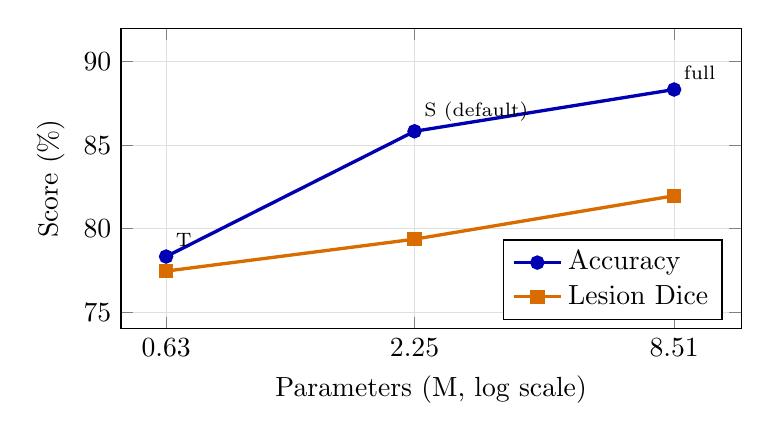
\begin{tikzpicture}
\begin{axis}[
  width=0.78\textwidth, height=5.4cm,
  xmode=log, log basis x=10,
  xtick={0.63,2.25,8.51}, xticklabels={0.63,2.25,8.51},
  xlabel={Parameters (M, log scale)}, ylabel={Score (\%)},
  xmin=0.5, xmax=12, ymin=74, ymax=92,
  legend pos=south east, legend cell align=left,
  grid=both, grid style={gray!25},
  every axis plot/.append style={very thick}]
\addplot[mark=*,color=blue!70!black] coordinates {(0.63,78.33) (2.25,85.83) (8.51,88.33)};
\addlegendentry{Accuracy}
\addplot[mark=square*,color=orange!85!black] coordinates {(0.63,77.46) (2.25,79.37) (8.51,81.97)};
\addlegendentry{Lesion Dice}
\node[anchor=south west,font=\scriptsize] at (axis cs:0.63,78.33) {T};
\node[anchor=south west,font=\scriptsize] at (axis cs:2.25,85.83) {S (default)};
\node[anchor=south west,font=\scriptsize] at (axis cs:8.51,88.33) {full};
\end{axis}
\end{tikzpicture}
\caption{Accuracy and lesion Dice versus parameter count for the DAMK-Net width
family (Table~\ref{tab:main}). DAMK-Net-S sits at the knee.}
\label{fig:pareto}
\end{figure}

\subsection{Per-class results and clinical false positives}
Table~\ref{tab:perclass} breaks the proposed model down by class. After refining,
normal segmentation reaches 0.81 Dice for DAMK-Net-S and 0.90 for the full model.
Classification F1 is balanced across the three classes, with malignant the
hardest at 0.81 and 0.79. Because flagging a healthy scan triggers unnecessary
follow-up, the clinically relevant number is the false-positive rate on normal
scans -- the fraction of normal images the model labels as containing a lesion.
Prediction-refining lowers this rate from 23.8\% to 14.3\% for DAMK-Net-S and from
14.3\% to 9.5\% for the full model, which raises specificity to 0.86 and 0.90.
Figure~\ref{fig:qual} shows representative test cases for the three classes: the
predicted mask follows the lesion boundary closely for benign and malignant
scans, and is correctly left empty for the normal scan.

\begin{figure}[t]
\centering
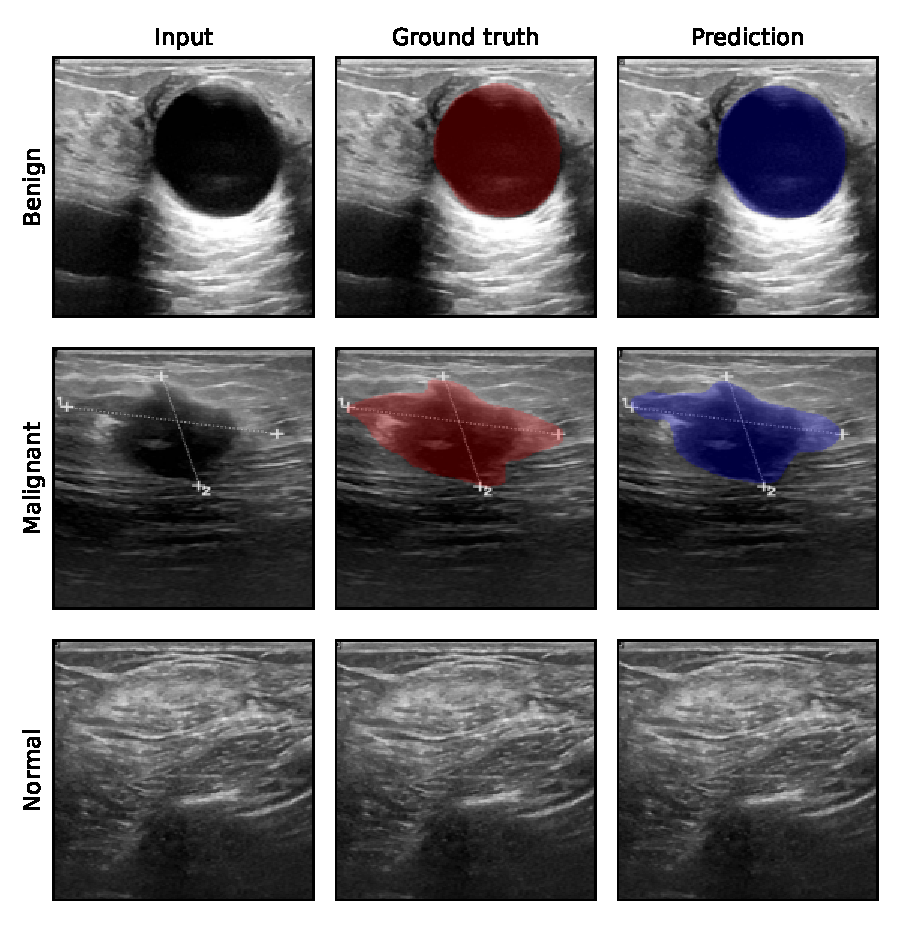
\includegraphics[width=0.78\textwidth]{fig3_qualitative}
\caption{Representative DAMK-Net (full) predictions on the BUSI test set, one per
class. Columns: input image, ground-truth mask, predicted mask (after
prediction-refining). The benign and malignant lesions are segmented accurately;
the normal scan yields an empty mask, as intended.}
\label{fig:qual}
\end{figure}

\begin{table}[t]
\caption{Per-class results for the proposed model (full OS+PR).}
\label{tab:perclass}
\centering
\begin{tabular}{lcc}
\toprule
Model & Dice (ben./mal./norm.) & F1 (ben./mal./norm.) \\
\midrule
DAMK-Net-S & 79.2 / 79.6 / 81.0 & 0.878 / 0.806 / 0.872 \\
DAMK-Net   & 82.3 / 81.3 / 90.5 & 0.903 / 0.786 / 0.950 \\
\bottomrule
\end{tabular}
\end{table}

\subsection{Threshold robustness and runtime}
The area threshold $\tau$ used by prediction-refining is selected on the
validation set. The refined metrics are stable across $\tau \in [0.0005, 0.005]$,
a tenfold range, and degrade only for $\tau \geq 0.01$
(Figure~\ref{fig:tau}), so the result does not
depend on a finely tuned value. On a CPU at batch size 1, DAMK-Net-T, DAMK-Net-S,
and the full model run at 37, 70, and 138 ms per image; latency grows with FLOPs
but more slowly, and the smallest variant stays within an interactive range
without a GPU.

\begin{figure}[t]
\centering
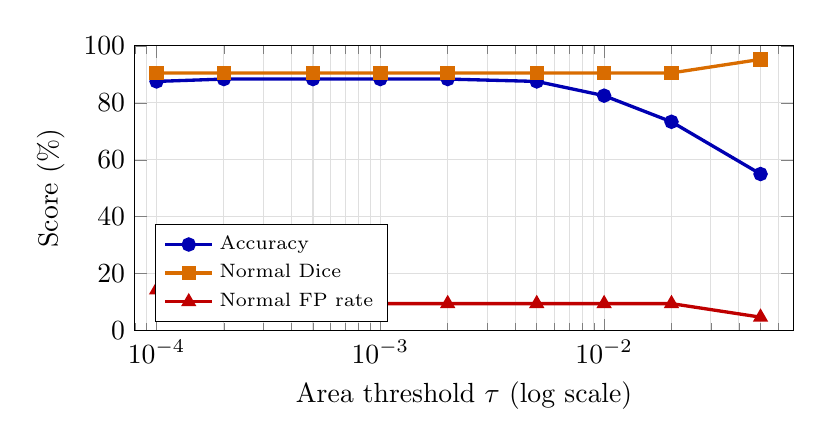
\begin{tikzpicture}
\begin{axis}[
  width=0.82\textwidth, height=5.2cm,
  xmode=log, log basis x=10,
  xlabel={Area threshold $\tau$ (log scale)}, ylabel={Score (\%)},
  xmin=8e-5, xmax=7e-2, ymin=0, ymax=100,
  legend pos=south west, legend cell align=left, legend style={font=\scriptsize},
  grid=both, grid style={gray!25},
  every axis plot/.append style={very thick}]
\addplot[mark=*,color=blue!70!black] coordinates {(0.0001,87.50) (0.0002,88.33) (0.0005,88.33) (0.001,88.33) (0.002,88.33) (0.005,87.50) (0.01,82.50) (0.02,73.33) (0.05,55.00)};
\addlegendentry{Accuracy}
\addplot[mark=square*,color=orange!85!black] coordinates {(0.0001,90.48) (0.0002,90.48) (0.0005,90.48) (0.001,90.48) (0.002,90.48) (0.005,90.48) (0.01,90.48) (0.02,90.48) (0.05,95.24)};
\addlegendentry{Normal Dice}
\addplot[mark=triangle*,color=red!75!black] coordinates {(0.0001,14.29) (0.0002,9.52) (0.0005,9.52) (0.001,9.52) (0.002,9.52) (0.005,9.52) (0.01,9.52) (0.02,9.52) (0.05,4.76)};
\addlegendentry{Normal FP rate}
\end{axis}
\end{tikzpicture}
\caption{Sensitivity of the full DAMK-Net to the prediction-refining area
threshold $\tau$ on the BUSI test set. Accuracy, normal-class Dice, and the
false-positive rate on normal scans are flat across the band
$\tau\in[5{\times}10^{-4},5{\times}10^{-3}]$; accuracy falls only once $\tau$
reaches $10^{-2}$, where genuine small lesions start being relabelled normal.}
\label{fig:tau}
\end{figure}

\section{Discussion}
The efficiency result points to the shared encoder as the reason a single model
undercuts the two-model pipeline. Both tasks need a strong feature extractor, and
they can use the same one, so the extra cost of adding segmentation to a
classifier is the decoder, not a second backbone. This is why DAMK-Net-S stays
below MedNet and MK-UNet run together while doing more than either. The same gap
separates DAMK-Net from the multi-task breast-ultrasound methods that keep the
joint setting: their backbones are an order of magnitude larger, from the 42.99M
parameters of ACSNet \cite{ACSNet} to the UNet++ and nnU-Net stages used by the
framework of Aumente-Maestro et al. \cite{CMPB}, whereas the DAMK-Net family runs
from 0.63M to 8.5M. We use these methods' published costs rather than re-running
them, since they target a different operating point; the structural argument for
the gap, a single shared encoder instead of heavy task-specific stages, does not
depend on the protocol.

The normal-class result holds beyond our specific network. Two output heads are
each trained to be accurate, not to agree with one another, so a multi-task model
is free to label a scan normal and still paint a lesion on it. Nothing in the
loss forbids that, and the numbers show it happening: the plain multi-task model
scores 0.43 on normal scans. Consistency between the heads has to be imposed
rather than assumed, and the inference-time step that imposes it is what moves the
normal class. A lightweight multi-task ultrasound model built without such a step
will keep flagging healthy tissue, which in screening means unnecessary
follow-up.

On a fixed encoder, the multi-kernel decoder reconstructs masks both better and
more cheaply than the inception-style decoder. Parallel small and large kernels
span the size range of lesions in one block, while the inception decoder pays for
a channel expansion it does not recover in accuracy. The gap, 79.4\% against
74.8\% Dice at a seventh of the compute, is large enough to settle the decoder
choice on this backbone. We do not match the dedicated segmenter on its own
ground, and the paper does not claim to. MK-UNet remains the lighter and equally
accurate option when segmentation is all that is required. The contribution is
completeness at low cost: one deployable model that classifies, segments, and
recognizes normal scans, together with an account of which components make that
combination work.

To see where the shared encoder looks, Figure~\ref{fig:gradcam} shows Grad-CAM
maps \cite{CBAM} from the final encoder stage for the same three cases. On the
benign and malignant scans the activation concentrates on the lesion, the region
the segmentation head also marks; on the normal scan it stays diffuse, with no
focal response, consistent with the empty mask. The maps are illustrative rather
than a quantitative claim, but they indicate that the features the two heads share
are lesion-centred.

\begin{figure}[t]
\centering
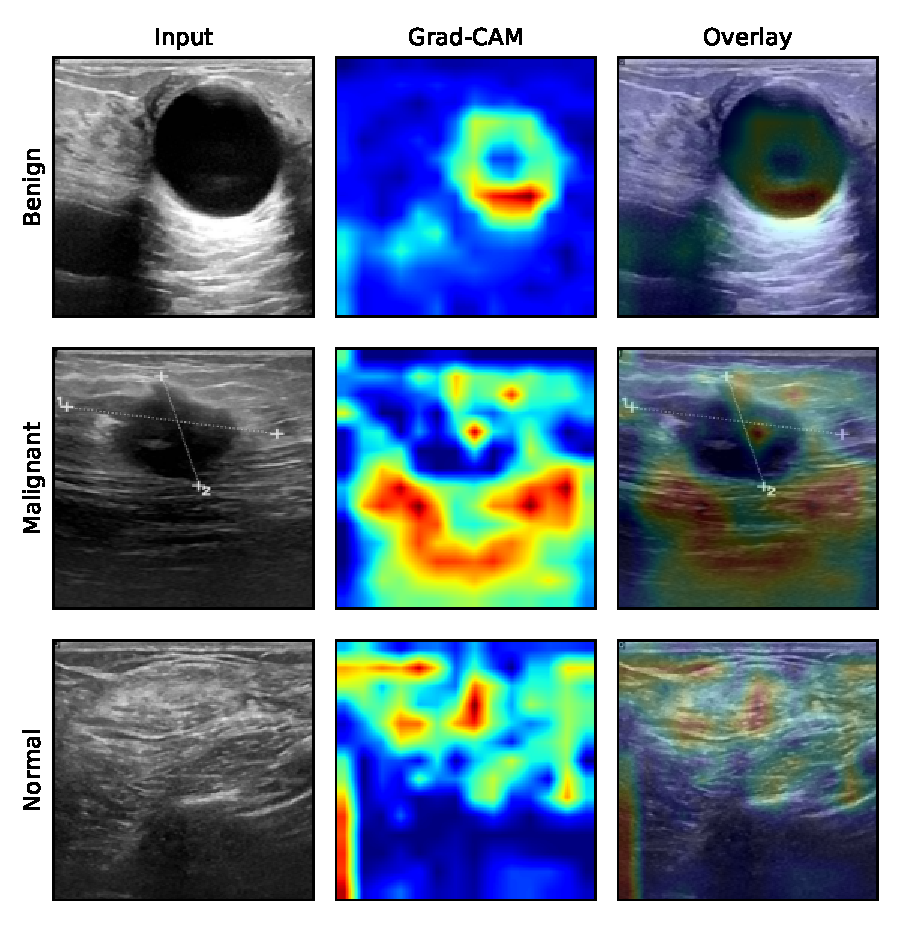
\includegraphics[width=0.78\textwidth]{fig5_gradcam}
\caption{Grad-CAM maps from the last encoder stage of DAMK-Net (full) for the
three cases of Figure~\ref{fig:qual}. Columns: input, Grad-CAM, overlay. The
response is lesion-centred for benign and malignant scans and diffuse for the
normal scan.}
\label{fig:gradcam}
\end{figure}

\section{Conclusion and Limitations}
DAMK-Net classifies and segments a breast ultrasound scan in one compact model
and keeps normal scans in the loop. At 2.25M parameters the DAMK-Net-S
configuration reaches classification accuracy above a dedicated classifier and
lesion Dice on par with a dedicated segmenter, below the cost of running both, and
a width multiplier exposes a family from 0.63M to 8.5M parameters. The ablations
show that handling normal scans depends on an explicit coherence step rather than
on the multi-task heads, and that a multi-kernel decoder is the efficient choice
on this encoder.

Several limits remain. The evaluation is on a single public dataset (BUSI), so
behavior on other scanners, vendors, and populations is untested; external
validation on an independent cohort is the clearest next step. Our comparison
against multi-task methods uses their published cost rather than a re-run under
our protocol, because those models are an order of magnitude larger and target a
different operating point; a same-protocol multi-task comparison is left to future
work. The smallest configuration trades accuracy for size and is not free.
Prediction-refining uses a fixed area threshold; although the result is stable
across a wide range of that threshold, a learned or adaptive criterion could
remove the hyper-parameter entirely and might handle small lesions better. The
oversampling and refining mechanisms are adapted from prior work, and our role is
their integration into a compact, scalable model and the analysis of their effect,
not the mechanisms themselves.

% \begin{credits}
% \subsubsection{\ackname} This research received no specific grant from funding
% agencies in the public, commercial, or not-for-profit sectors.

% \subsubsection{\discintname}
% The authors have no competing interests to declare that are relevant to the
% content of this article.
% \end{credits}

\begin{thebibliography}{33}

\bibitem{ACSNet}
He, Q., Yang, Q., Su, H., Wang, Y.: Multi-task learning for segmentation and classification of breast tumors from ultrasound images. Comput. Biol. Med. \textbf{173}, 108319 (2024)

\bibitem{AttnUNet}
Oktay, O., Schlemper, J., Folgoc, L.L., Lee, M., Heinrich, M.P., Misawa, K., Mori, K., McDonagh, S., Hammerla, N.Y., Kainz, B., Glocker, B., Rueckert, D.: Attention U-Net: learning where to look for the pancreas. CoRR abs/1804.03999 (2018)

\bibitem{BUSI}
Al-Dhabyani, W., Gomaa, M., Khaled, H., Fahmy, A.: Dataset of breast ultrasound images. Data in Brief \textbf{28}, 104863 (2020)

\bibitem{CBAM}
Woo, S., Park, J., Lee, J.Y., Kweon, I.S.: CBAM: convolutional block attention module. In: ECCV, pp. 3--19 (2018)

\bibitem{CMPB}
Aumente-Maestro, C., Díez, J., Remeseiro, B.: A multi-task framework for breast cancer segmentation and classification in ultrasound imaging. Comput. Biol. Med. \textbf{260}, 108540 (2025)

\bibitem{CMUNeXt}
Tang, F., Ding, J., Quan, Q., Wang, L., Ning, C., Zhou, S.K.: CMUNeXt: an efficient medical image segmentation network based on large kernel and skip fusion. In: IEEE ISBI, pp. 1--5 (2024)

\bibitem{DBL}
Zhu, C., et al.: DBL-Net: a dual-branch learning network with information from spatial and frequency domains for tumor segmentation and classification in breast ultrasound image. Biomed. Signal Process. Control \textbf{93}, 106221 (2024)

\bibitem{DSN}
Lee, C.Y., Xie, S., Gallagher, P., Zhang, Z., Tu, Z.: Deeply-supervised nets. In: AISTATS, pp. 562--570 (2015)

\bibitem{EGEUNet}
Ruan, J., Xie, M., Gao, J., Liu, T., Fu, Y.: EGE-UNet: an efficient group enhanced UNet for skin lesion segmentation. In: MICCAI, pp. 481--490 (2023)

\bibitem{Focal}
Lin, T.Y., Goyal, P., Girshick, R., He, K., Dollár, P.: Focal loss for dense object detection. In: IEEE ICCV, pp. 2980--2988 (2017)

\bibitem{GGN}
Xue, C., Zhu, L., Fu, H., Hu, X., Li, X., Zhang, H., Heng, P.A.: Global guidance network for breast lesion segmentation in ultrasound images. Med. Image Anal. \textbf{70}, 101989 (2021)

\bibitem{Globocan}
Sung, H., et al.: Global cancer statistics 2020: GLOBOCAN estimates of incidence and mortality worldwide for 36 cancers in 185 countries. CA Cancer J. Clin. \textbf{71}(3), 209--249 (2021)

\bibitem{HCTNet}
He, Q., Yang, Q., Xie, M.: HCTNet: a hybrid CNN-transformer network for breast ultrasound image segmentation. Comput. Biol. Med. \textbf{155}, 106629 (2023)

\bibitem{HoVerTrans}
Mo, Y., Han, C., et al.: HoVer-Trans: anatomy-aware HoVer-transformer for ROI-free breast cancer diagnosis in ultrasound images. IEEE Trans. Med. Imaging \textbf{42}(6), 1696--1706 (2023)

\bibitem{MADTNet}
Ghosh, S., Das, S.: Enhancing medical image analysis with MA-DTNet: a dual task network guided by morphological attention. In: ICPR. LNCS (2024). doi:10.1007/978-3-031-78198-8\_19

\bibitem{MALUNet}
Ruan, J., Xiang, S., Xie, M., Liu, T., Fu, Y.: MALUNet: a multi-attention and light-weight UNet for skin lesion segmentation. In: IEEE BIBM, pp. 1150--1156 (2022)

\bibitem{MKUNet}
Rahman, M.M., Marculescu, R.: MK-UNet: multi-kernel lightweight CNN for medical image segmentation. In: IEEE/CVF ICCV Workshops, pp. 1053--1062 (2024)

\bibitem{MedNet}
Ferdous, M., Mahmud, S., Shimul, M.E.Z.: MedNet: a lightweight attention-augmented CNN for medical image classification. Sci. Rep. \textbf{15}, 41936 (2025)

\bibitem{MobileNet}
Howard, A.G., et al.: MobileNets: efficient convolutional neural networks for mobile vision applications. arXiv:1704.04861 (2017)

\bibitem{MobileNetV2}
Sandler, M., Howard, A., Zhu, M., Zhmoginov, A., Chen, L.C.: MobileNetV2: inverted residuals and linear bottlenecks. In: IEEE CVPR, pp. 4510--4520 (2018)

\bibitem{RMTLNet}
Xu, M., Huang, K., Qi, X.: A regional-attentive multi-task learning framework for breast ultrasound image segmentation and classification. IEEE Access \textbf{11}, 5377--5392 (2023)

\bibitem{SENet}
Hu, J., Shen, L., Sun, G.: Squeeze-and-excitation networks. In: IEEE CVPR, pp. 7132--7141 (2018)

\bibitem{SHAMTL}
Zhang, G., Zhao, K., Hong, Y., Qiu, X., Zhang, K., Wei, B.: SHA-MTL: soft and hard attention multi-task learning for automated breast cancer ultrasound image segmentation and classification. Int. J. Comput. Assist. Radiol. Surg. \textbf{16}, 1719--1725 (2021)

\bibitem{Shareef}
Shareef, B., Xian, M., Vakanski, A., Wang, H.: Breast ultrasound tumor classification using a hybrid multitask CNN-transformer network. In: MICCAI, pp. 344--353 (2023)

\bibitem{ShuffleNet}
Zhang, X., Zhou, X., Lin, M., Sun, J.: ShuffleNet: an extremely efficient convolutional neural network for mobile devices. In: IEEE CVPR, pp. 6848--6856 (2018)

\bibitem{Survey}
Liu, J., Pian, L., Chen, J., Zhao, J., Liu, Y., Meng, F., Zeng, C.: Artificial intelligence in breast ultrasound: a systematic review of research advances. Front. Oncol. \textbf{15}, 1619364 (2025)

\bibitem{UNeXt}
Valanarasu, J.M.J., Patel, V.M.: UNeXt: MLP-based rapid medical image segmentation network. In: MICCAI, pp. 23--33 (2022)

\bibitem{UNet}
Ronneberger, O., Fischer, P., Brox, T.: U-Net: convolutional networks for biomedical image segmentation. In: MICCAI (3), pp. 234--241 (2015)

\bibitem{UNetpp}
Zhou, Z., Rahman Siddiquee, M.M., Tajbakhsh, N., Liang, J.: UNet++: a nested U-Net architecture for medical image segmentation. In: DLMIA Workshop, MICCAI, pp. 3--11 (2018)

\bibitem{VMUNet}
Wu, R., Liu, Y., Liang, P., Chang, Q.: UltraLight VM-UNet: parallel vision Mamba significantly reduces parameters for skin lesion segmentation. arXiv:2403.20035 (2024)

\bibitem{VNet}
Milletari, F., Navab, N., Ahmadi, S.A.: V-Net: fully convolutional neural networks for volumetric medical image segmentation. In: 3DV, pp. 565--571 (2016)

\bibitem{Xception}
Chollet, F.: Xception: deep learning with depthwise separable convolutions. In: IEEE CVPR, pp. 1251--1258 (2017)

\bibitem{Zhou}
Zhou, Y., et al.: Multi-task learning for segmentation and classification of tumors in 3D automated breast ultrasound images. Med. Image Anal. \textbf{70}, 101918 (2021)

\end{thebibliography}

% \begin{thebibliography}{33}
% \bibitem{ACSNet}
% He, Q., Yang, Q., Su, H., Wang, Y.: Multi-task learning for segmentation and
% classification of breast tumors from ultrasound images. Comput. Biol. Med.
% \textbf{173}, 108319 (2024)

% \bibitem{AttnUNet}
% Oktay, O., et al.: Attention U-Net: learning where to look for the pancreas. In:
% MIDL (2018). arXiv:1804.03999

% \bibitem{BUSI}
% Al-Dhabyani, W., Gomaa, M., Khaled, H., Fahmy, A.: Dataset of breast ultrasound
% images. Data in Brief \textbf{28}, 104863 (2020)

% \bibitem{CBAM}
% Woo, S., Park, J., Lee, J.Y., Kweon, I.S.: CBAM: convolutional block attention
% module. In: ECCV, pp. 3--19 (2018)

% \bibitem{CMPB}
% Aumente-Maestro, C., D\'iez, J., Remeseiro, B.: A multi-task framework for breast
% cancer segmentation and classification in ultrasound imaging. Comput. Biol. Med.
% \textbf{260}, 108540 (2025)

% \bibitem{CMUNeXt}
% Tang, F., Ding, J., Quan, Q., Wang, L., Ning, C., Zhou, S.K.: CMUNeXt: an
% efficient medical image segmentation network based on large kernel and skip
% fusion. In: IEEE ISBI, pp. 1--5 (2024)

% \bibitem{DBL}
% Zhu, C., et al.: DBL-Net: a dual-branch learning network with information from
% spatial and frequency domains for tumor segmentation and classification in breast
% ultrasound image. Biomed. Signal Process. Control \textbf{93}, 106221 (2024)

% \bibitem{DSN}
% Lee, C.Y., Xie, S., Gallagher, P., Zhang, Z., Tu, Z.: Deeply-supervised nets. In:
% AISTATS, pp. 562--570 (2015)

% \bibitem{EGEUNet}
% Ruan, J., Xie, M., Gao, J., Liu, T., Fu, Y.: EGE-UNet: an efficient group enhanced
% UNet for skin lesion segmentation. In: MICCAI, pp. 481--490 (2023)

% \bibitem{Focal}
% Lin, T.Y., Goyal, P., Girshick, R., He, K., Doll\'ar, P.: Focal loss for dense
% object detection. In: IEEE ICCV, pp. 2980--2988 (2017)

% \bibitem{GGN}
% Xue, C., Zhu, L., Fu, H., Hu, X., Li, X., Zhang, H., Heng, P.A.: Global guidance
% network for breast lesion segmentation in ultrasound images. Med. Image Anal.
% \textbf{70}, 101989 (2021)

% \bibitem{Globocan}
% Sung, H., et al.: Global cancer statistics 2020: GLOBOCAN estimates of incidence
% and mortality worldwide for 36 cancers in 185 countries. CA Cancer J. Clin.
% \textbf{71}(3), 209--249 (2021)

% \bibitem{HCTNet}
% He, Q., Yang, Q., Xie, M.: HCTNet: a hybrid CNN-transformer network for breast
% ultrasound image segmentation. Comput. Biol. Med. \textbf{155}, 106629 (2023)

% \bibitem{HoVerTrans}
% Mo, Y., Han, C., et al.: HoVer-Trans: anatomy-aware HoVer-transformer for ROI-free
% breast cancer diagnosis in ultrasound images. IEEE Trans. Med. Imaging
% \textbf{42}(6), 1696--1706 (2023)

% \bibitem{MADTNet}
% Ghosh, S., Das, S.: Enhancing medical image analysis with MA-DTNet: a dual task
% network guided by morphological attention. In: ICPR. LNCS, Springer (2024).
% \doi{10.1007/978-3-031-78198-8\_19}

% \bibitem{MALUNet}
% Ruan, J., Xiang, S., Xie, M., Liu, T., Fu, Y.: MALUNet: a multi-attention and
% light-weight UNet for skin lesion segmentation. In: IEEE BIBM, pp. 1150--1156
% (2022)

% \bibitem{MKUNet}
% Rahman, M.M., Marculescu, R.: MK-UNet: multi-kernel lightweight CNN for medical
% image segmentation. In: IEEE/CVF ICCV Workshops, pp. 1053--1062 (2024)

% \bibitem{MedNet}
% Ferdous, M., Mahmud, S., Shimul, M.E.Z.: MedNet: a lightweight attention-augmented
% CNN for medical image classification. Sci. Rep. \textbf{15}, 41936 (2025)

% \bibitem{MobileNet}
% Howard, A.G., et al.: MobileNets: efficient convolutional neural networks for
% mobile vision applications. arXiv:1704.04861 (2017)

% \bibitem{MobileNetV2}
% Sandler, M., Howard, A., Zhu, M., Zhmoginov, A., Chen, L.C.: MobileNetV2: inverted
% residuals and linear bottlenecks. In: IEEE CVPR, pp. 4510--4520 (2018)

% \bibitem{RMTLNet}
% Xu, M., Huang, K., Qi, X.: A regional-attentive multi-task learning framework for
% breast ultrasound image segmentation and classification. IEEE Access \textbf{11},
% 5377--5392 (2023)

% \bibitem{SENet}
% Hu, J., Shen, L., Sun, G.: Squeeze-and-excitation networks. In: IEEE CVPR, pp.
% 7132--7141 (2018)

% \bibitem{SHAMTL}
% Zhang, G., Zhao, K., Hong, Y., Qiu, X., Zhang, K., Wei, B.: SHA-MTL: soft and hard
% attention multi-task learning for automated breast cancer ultrasound image
% segmentation and classification. Int. J. Comput. Assist. Radiol. Surg.
% \textbf{16}, 1719--1725 (2021)

% \bibitem{Shareef}
% Shareef, B., Xian, M., Vakanski, A., Wang, H.: Breast ultrasound tumor
% classification using a hybrid multitask CNN-transformer network. In: MICCAI, pp.
% 344--353 (2023)

% \bibitem{ShuffleNet}
% Zhang, X., Zhou, X., Lin, M., Sun, J.: ShuffleNet: an extremely efficient
% convolutional neural network for mobile devices. In: IEEE CVPR, pp. 6848--6856
% (2018)

% \bibitem{Survey}
% Liu, J., Pian, L., Chen, J., Zhao, J., Liu, Y., Meng, F., Zeng, C.: Artificial
% intelligence in breast ultrasound: a systematic review of research advances.
% Front. Oncol. \textbf{15}, 1619364 (2025)

% \bibitem{UNeXt}
% Valanarasu, J.M.J., Patel, V.M.: UNeXt: MLP-based rapid medical image segmentation
% network. In: MICCAI, pp. 23--33 (2022)

% \bibitem{UNet}
% Ronneberger, O., Fischer, P., Brox, T.: U-Net: convolutional networks for
% biomedical image segmentation. In: MICCAI, pp. 234--241 (2015)

% \bibitem{UNetpp}
% Zhou, Z., Rahman Siddiquee, M.M., Tajbakhsh, N., Liang, J.: UNet++: a nested U-Net
% architecture for medical image segmentation. In: DLMIA Workshop, MICCAI, pp.
% 3--11 (2018)

% \bibitem{VMUNet}
% Wu, R., Liu, Y., Liang, P., Chang, Q.: UltraLight VM-UNet: parallel vision Mamba
% significantly reduces parameters for skin lesion segmentation. arXiv:2403.20035
% (2024)

% \bibitem{VNet}
% Milletari, F., Navab, N., Ahmadi, S.A.: V-Net: fully convolutional neural networks
% for volumetric medical image segmentation. In: 3DV, pp. 565--571 (2016)

% \bibitem{Xception}
% Chollet, F.: Xception: deep learning with depthwise separable convolutions. In:
% IEEE CVPR, pp. 1251--1258 (2017)

% \bibitem{Zhou}
% Zhou, Y., et al.: Multi-task learning for segmentation and classification of
% tumors in 3D automated breast ultrasound images. Med. Image Anal. \textbf{70},
% 101918 (2021)
% \end{thebibliography}
\end{document}
